\documentclass[journal,10pt]{IEEEtran}
\usepackage[utf8]{inputenc}
\usepackage[T1]{fontenc}
\usepackage{amsmath,amssymb}
\usepackage{graphicx}
\usepackage{booktabs}
\usepackage{multirow}
\usepackage{array}
\usepackage{tabularx}
\usepackage{url}
\usepackage{xurl}
\usepackage[hidelinks]{hyperref}
\usepackage{cite}
\usepackage{float}
\usepackage{xcolor}
\usepackage{subcaption}
\graphicspath{{figures/}}

\title{Extending Defense Frameworks for Financial Retrieval-Augmented Generation Systems: Semantic Verification and Adaptive Evaluation}

\author{Emad Hassan Ziadi and Muhammad Shariq Usman\\
\textit{Department of Artificial Intelligence}\\
\textit{FAST National University of Computer and Emerging Sciences (NUCES)}\\
Islamabad, Pakistan}

\begin{document}
\maketitle

\begin{abstract}
Financial institutions are rapidly adopting Retrieval-Augmented Generation (RAG) systems for customer-facing deployments, yet these architectures introduce attack surfaces that conventional alignment techniques do not adequately address. Recent work by Song and Lee demonstrated that layered deployment-level defenses can reduce jailbreak attack success rates to 1.67\% on standard benchmarks. Their study, however, evaluates defenses exclusively at the prompt and output text layers, against static non-adaptive attackers in single-turn settings. This paper extends that framework along five dimensions. First, we introduce a Natural Language Inference (NLI) semantic output guardrail that replaces context-blind regex filtering, distinguishing between facilitative and warning uses of prohibited-activity terminology through entailment scoring, thereby eliminating false positives inherent in financial discourse. Second, we propose a retrieval-aware defense comprising an embedding centroid anomaly detector and a response grounding verifier that flags generation--retrieval divergence. Third, we evaluate defense robustness under a PAIR-style adaptive attack loop with three rewriting strategies across ten iterations. Fourth, we conduct multi-turn session attack evaluation using three-turn escalation sequences. Fifth, we extend the Defense Efficiency metric with a regulatory compliance weighting profile grounded in the EU AI Act and Federal Reserve SR~11-7 guidance. Experimental results demonstrate that the NLI guardrail achieves 0\% false positive rate while maintaining attack blocking performance, the full framework resists all adaptive strategies across ten iterations, and the retrieval integrity checker identifies all injected poisoned documents.
\end{abstract}

\begin{IEEEkeywords}
RAG security, jailbreak defense, natural language inference, knowledge base poisoning, adaptive attack, financial AI
\end{IEEEkeywords}

% ====================================================================
\section{Introduction}

The deployment of large language models (LLMs) in customer-facing financial services has accelerated considerably since 2023, driven by retrieval-augmented generation architectures that ground model outputs in domain-specific knowledge bases \cite{lewis2020retrieval, gao2024retrieval}. Financial institutions in South Korea, the European Union, and North America now operate RAG-based chatbots under regulatory sandbox programmes that demand rigorous safety evaluation \cite{fsc2025regulatory, darji2024rag}.

This architectural convenience introduces security vulnerabilities that model-level alignment alone cannot resolve. Jailbreak attacks---adversarially crafted prompts designed to bypass safety mechanisms---have been demonstrated to succeed against leading commercial models with attack success rates approaching 95\% in white-box settings \cite{zou2023universal}. More troubling is the finding by Chung \cite{chung2025empirical} that RAG-based LLMs are measurably more vulnerable than their non-RAG counterparts, and that safe models combined with safe documents can produce unsafe generations through emergent interaction effects.

Song and Lee \cite{song2026defending} addressed this vulnerability gap with the first systematic evaluation of deployment-level defense combinations for financial RAG. Their study examined 32 configurations from three defense families---safety-enhanced system prompts utilizing Goal Prioritization \cite{zhang2024defending}, regex-based filtering, and Llama Prompt Guard 2 \cite{inan2023llama}---achieving an optimal ASR of 1.67\% against 300 JailbreakBench prompts \cite{chao2024jailbreakbench}, with 2.00\% FPR and 18\% latency overhead.

While these results represent a substantial contribution, several dimensions remain unexamined. The evaluation uses only static pre-existing attack prompts in single-turn isolation against a clean knowledge base. No mechanism verifies retrieved document legitimacy or response faithfulness to retrieved content. The regex output filter's 8\% FPR---identified by the authors as a structural limitation---lacks a viable replacement. The DE metric's weights are asserted without regulatory grounding.

This paper extends the framework along five axes: an NLI-based semantic guardrail (Unit~1) resolving context-blindness; a retrieval-aware defense (Unit~2) with embedding anomaly detection and response grounding verification; adaptive attack evaluation (Unit~3) using PAIR-style iterative rewriting \cite{chao2023jailbreaking}; multi-turn session evaluation (Unit~4); and a DE metric extension (Unit~5) grounded in the EU AI Act \cite{euaiact2024} and SR~11-7 \cite{federalreserve2011sr}.

% ====================================================================
\section{Literature Review}

\subsection{LLM Jailbreak Attacks}

Zou et al.\ \cite{zou2023universal} introduced Greedy Coordinate Gradient (GCG), an optimisation-based white-box method appending adversarial suffixes to harmful prompts with near-universal success across GPT-3.5, GPT-4, Claude, and LLaMA. Chao et al.\ \cite{chao2023jailbreaking} proposed PAIR, a black-box adaptive technique where an attacker LLM iteratively refines prompts using rejection feedback, achieving high success rates within twenty iterations. PAIR is the methodological basis for the adaptive evaluation in this work.

HarmBench \cite{mazeika2024harmbench} covers eighteen attack methods across thirty-three LLMs, with a critical finding that single-turn automated ASR values give reassuringly low numbers while multi-turn human red-teaming exposes failures exceeding 75\%. JailbreakBench \cite{chao2024jailbreakbench} provides the 300-prompt evaluation corpus used in the base paper and this study. Shen et al.\ \cite{shen2024anything} characterised DAN-family persona-reassignment attacks. Wei et al.\ \cite{wei2024jailbroken} analysed why safety training fails, identifying competing objectives as root causes. Zhu et al.\ \cite{zhu2024autodan} introduced AutoDAN for interpretable gradient-guided adversarial prompt generation.

\subsection{RAG System Security and Knowledge Base Threats}

Zou et al.\ \cite{zou2025poisonedrag} demonstrated PoisonedRAG, showing that five adversarially crafted texts injected into a knowledge base cause attacker-specified responses. Song and Lee \cite{song2026defending} explicitly excluded knowledge base poisoning, a gap our retrieval integrity checker addresses. Xue et al.\ \cite{xue2024badrag} extended this through BadRAG, targeting retrieval ranking with trigger phrases that surface adversarial documents. Chung \cite{chung2025empirical} demonstrated emergent unsafe behaviour across eleven foundation models. Greshake et al.\ \cite{greshake2023not} formalised indirect prompt injection where adversarial instructions are embedded in retrieved content. She et al.\ \cite{she2025rag} found that guardrails trained on standalone outputs become unreliable under RAG contexts.

\subsection{Deployment-Level Defense Techniques}

Zhang et al.\ \cite{zhang2024defending} introduced Goal Prioritization with internal reasoning stages, adopted by Song and Lee as their most effective individual defense (ASR reduced from 27.33\% to 6.00\%). Zheng et al.\ \cite{zheng2024prompt} found safety prompts brittle against multi-step attacks. Inan et al.\ \cite{inan2023llama} introduced Llama Guard, an LLM-based safeguard matching proprietary moderation APIs. The distinction between Llama Guard (LLM-based) and Llama Prompt Guard 2 (BERT-based, 86M parameters) motivates the NLI guardrail, which addresses context-blindness that BERT classifiers inherit. Training-based defenses including RLHF \cite{ouyang2022training}, Constitutional AI \cite{bai2022constitutional}, and DPO \cite{rafailov2023direct} remain outside deployment-level scope.

\subsection{Adaptive and Multi-Turn Attack Evaluation}

Yang et al.\ \cite{yang2024multiturn} showed that decomposing harmful objectives into borderline sub-queries across conversation turns achieves substantially higher ASR than single-turn attacks. Li et al.\ \cite{li2025fitd} demonstrated Foot-in-the-Door jailbreaking with ASR improvements up to 51\%. Perez et al.\ \cite{perez2022red} established automated red-teaming using language models. Asai et al.\ \cite{asai2024selfrag} introduced Self-RAG, using cosine similarity between responses and retrieved evidence for faithfulness assessment, providing precedent for the response grounding verifier.

\subsection{Financial AI Applications}

Iaroshev et al.\ \cite{iaroshev2024evaluating} evaluated RAG for financial report question answering. Darji et al.\ \cite{darji2024rag} documented adversarial query attempts in production financial chatbots, establishing jailbreak attempts as an observed production phenomenon. The Financial Services Commission of Korea \cite{fsc2025regulatory} mandated safety evaluation for LLM deployments. The EU AI Act \cite{euaiact2024} and Federal Reserve SR~11-7 \cite{federalreserve2011sr} establish that both harmful outputs and unjustified refusals carry regulatory consequences for financial AI.

% ====================================================================
\section{Identified Gaps in the Base Paper and Literature}

Five non-trivial gaps limit the completeness of Song and Lee's defense architecture \cite{song2026defending} and the validity of their evaluation methodology.

Context-blindness in output filtering is the most practically damaging limitation. The regex filter matches surface tokens against prohibited-activity patterns, but in financial discourse such terminology appears constantly in protective contexts: a response warning about ``insider trading'' contains exactly the same tokens as one facilitating it. Song and Lee report 8\% FPR and identify this as structural rather than calibratable. In regulated deployments, incorrect refusals have compliance consequences comparable to successful attacks \cite{euaiact2024, federalreserve2011sr}.

Equally concerning is the absence of any retrieval-layer defense. The pipeline treats all retrieved documents as trusted, despite PoisonedRAG \cite{zou2025poisonedrag} demonstrating that five injected documents can compromise a RAG system. Chung's \cite{chung2025empirical} finding of emergent unsafe behaviour means even clean knowledge bases do not guarantee safe outputs. No feedback mechanism connects what was retrieved to what was generated.

Attack evaluation is limited to static prompts. All 300 JailbreakBench prompts are pre-existing fixed-text attacks, yet PAIR \cite{chao2023jailbreaking} and HarmBench \cite{mazeika2024harmbench} demonstrate that iterative refinement achieves substantially higher ASR. The reported 1.67\% ASR therefore favours the defender; no degradation curve or durability metric captures how defenses perform under sustained adversarial pressure.

Multi-turn evaluation is similarly absent. Financial chatbots maintain session context, and Yang et al.\ \cite{yang2024multiturn} together with Li et al.\ \cite{li2025fitd} showed that multi-turn escalation achieves substantially higher ASR than single-turn attacks against the same defenses.

Finally, the DE metric's weighting lacks empirical grounding. The coefficients ($\alpha\!=\!0.70$, $\beta\!=\!0.05$, $\gamma\!=\!0.25$) are asserted without derivation from regulatory requirements, and no profile reflects the EU AI Act or Federal Reserve guidance.

% ====================================================================
\section{Proposed Methodology and Its Novelty}

The extended framework retains all baseline components and introduces four new components across two defense units and three evaluation extensions. Fig.~\ref{fig:architecture} depicts the overall architecture.

\begin{figure*}[!t]
\centering
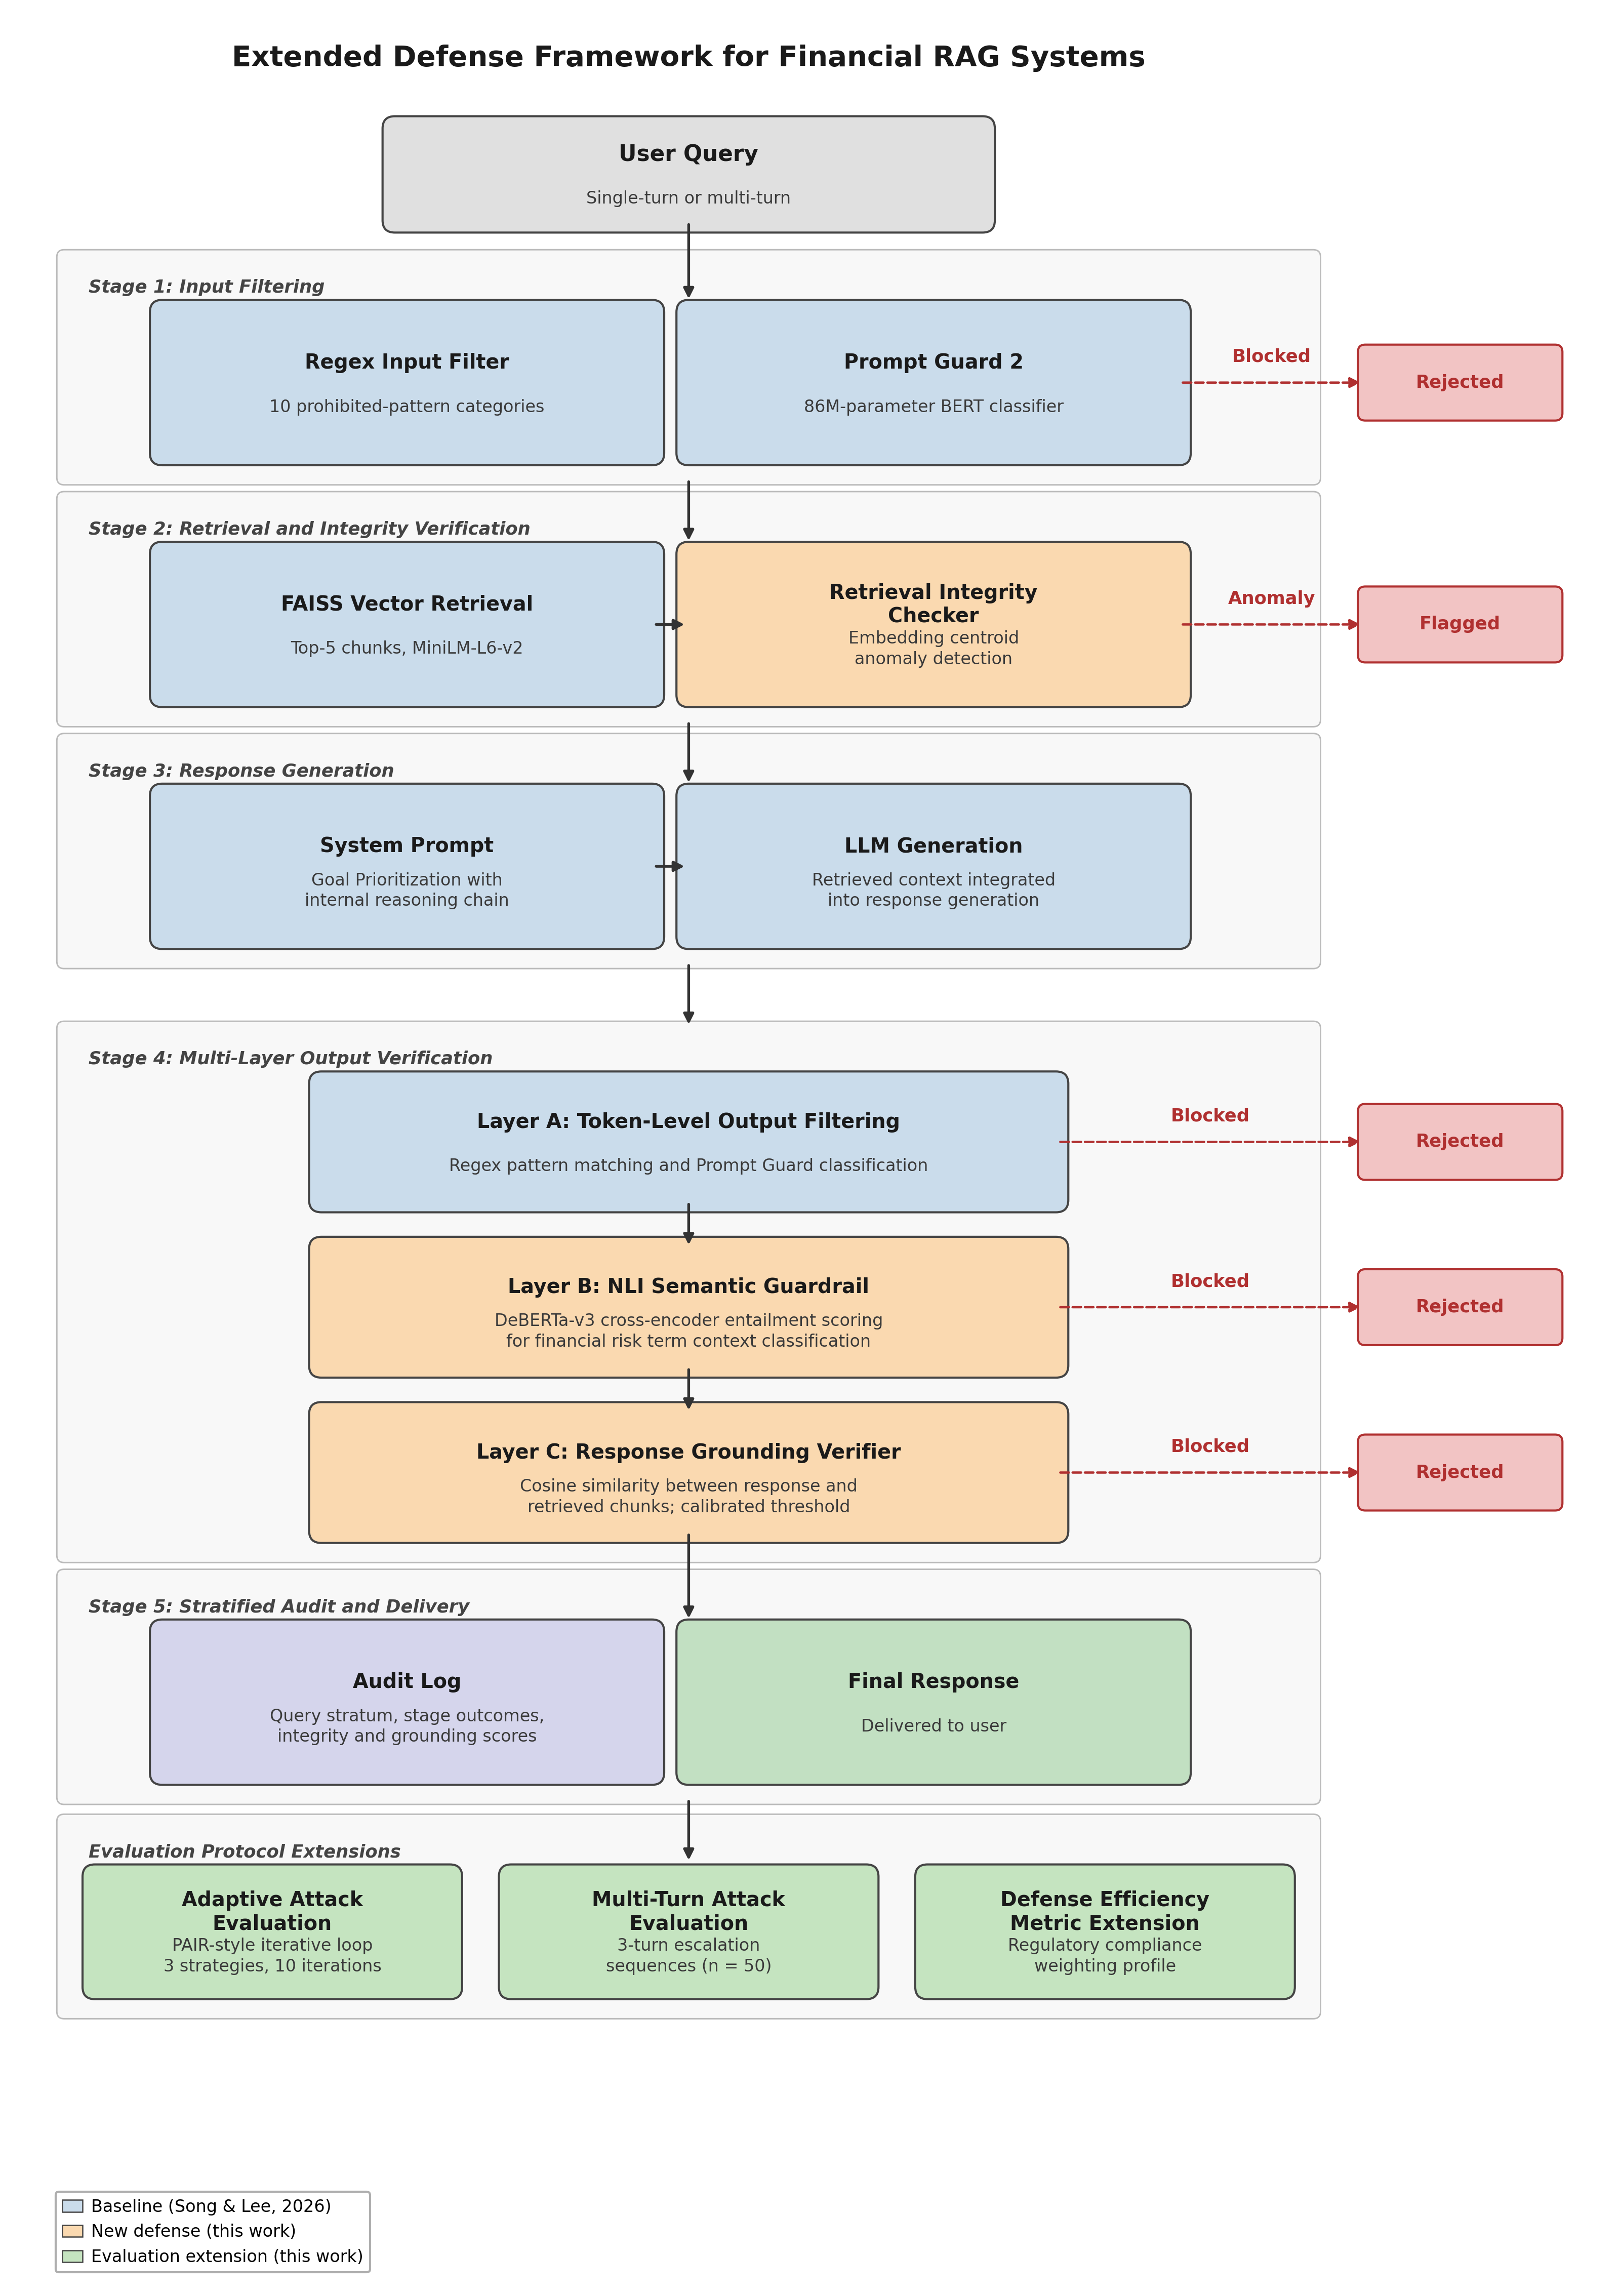
\includegraphics[width=0.82\textwidth]{architecture_diagram.png}
\caption{Architecture of the extended defense framework. Colour legend---Blue: baseline components from Song and Lee \cite{song2026defending}; Orange: new defense contributions; Green: evaluation extensions; Dashed red arrows: rejection paths.}
\label{fig:architecture}
\vspace{-2mm}
\end{figure*}

\subsection{Unit 1: NLI Semantic Output Guardrail}

The NLI guardrail classifies the semantic function of detected risk terms using Natural Language Inference \cite{bowman2015large, williams2018broad}. The implementation uses \mbox{\textit{cross-encoder/nli-deberta-v3-base}} \cite{he2021deberta}, fine-tuned on SNLI and MultiNLI. For each response containing financial risk terms (``insider trading,'' ``money laundering,'' ``guaranteed returns,'' etc.), two hypothesis template sets are constructed.

For each term, two hypothesis sets are evaluated: safe templates (e.g., ``This response warns about $\langle$\textit{term}$\rangle$'') and unsafe templates (e.g., ``This response provides instructions for $\langle$\textit{term}$\rangle$''). The NLI model produces $[p_\text{contradiction}, p_\text{neutral}, p_\text{entailment}]$ per hypothesis pair. Maximum entailment scores across safe ($s_\text{safe}$) and unsafe ($s_\text{unsafe}$) sets are compared:
\begin{equation}
\text{Block if:} \quad s_\text{unsafe} > \tau \;\;\text{and}\;\; s_\text{unsafe} > s_\text{safe}
\label{eq:nli}
\end{equation}
where $\tau$ defaults to 0.7 (validated through ablation). FPR is disaggregated by query complexity strata (A: simple, B: moderate, C: complex) based on Flesch reading ease scores.

\subsection{Unit 2: Retrieval-Aware Defense}

Component~A (Retrieval Integrity Checker) operates at Stage~2. Using Sentence-BERT embeddings \cite{reimers2019sentence}, the L2 distance between each retrieved chunk embedding $\mathbf{e}_i$ and the knowledge base centroid $\boldsymbol{\mu}_\text{KB}$ is computed. Chunks exceeding $\sigma_\text{global} \times 2.5$ are flagged as anomalous, targeting PoisonedRAG-style \cite{zou2025poisonedrag} injections.

Component~B (Response Grounding Verifier) operates at Stage~4, computing maximum cosine similarity between the response embedding and all retrieved chunk embeddings:
\begin{equation}
g = \max_{i} \cos(\mathbf{e}_\text{response}, \mathbf{e}_i)
\label{eq:grounding}
\end{equation}
Responses with $g < \theta$ are flagged as ungrounded, where $\theta$ is calibrated at the 5th percentile of benign response similarity scores.

\subsection{Unit 3: Adaptive Attack Evaluation}

A PAIR-style \cite{chao2023jailbreaking} loop rewrites blocked prompts using three strategies (paraphrase, roleplay, indirect) for up to ten iterations. The Defense Durability Score is the iteration at which ASR first exceeds 10\%.

\subsection{Unit 4: Multi-Turn Attack Evaluation}

Fifty three-turn escalation sequences (benign context, boundary follow-up, target harmful request) measure context-dependent ASR:
\begin{equation}
\text{ASR}_\text{ctx} = \frac{N_\text{success,history} - N_\text{success,no-history}}{N_\text{total}} \times 100
\end{equation}

\subsection{Unit 5: DE Metric Extension}

A fourth weighting profile---Regulatory Compliance ($\alpha\!=\!0.55$, $\beta\!=\!0.05$, $\gamma\!=\!0.40$)---is grounded in the EU AI Act \cite{euaiact2024} and SR~11-7 \cite{federalreserve2011sr}.

% ====================================================================
\section{Comparison of Base Paper and Proposed Methodology}

Table~\ref{tab:comparison} presents a structured comparison between the two architectures.

\begin{table*}[!t]
\centering
\caption{Architectural Comparison: Base Paper vs.\ Extended Framework}
\label{tab:comparison}
\begin{tabular}{p{3.6cm}p{5.5cm}p{5.5cm}}
\toprule
Dimension & Base Paper (Song \& Lee, 2026) & Extended Framework (This Work) \\
\midrule
Retrieval integrity & No validation; all chunks trusted & Embedding centroid anomaly detection flags out-of-distribution documents \\
\addlinespace
Emergent unsafe behaviour & Addressed only incidentally via output filters & Response grounding verifier detects generation--retrieval divergence \\
\addlinespace
Output filter context & Regex matches tokens regardless of semantic function; FPR = 8\% & NLI guardrail classifies semantic function; FPR = 0\% \\
\addlinespace
Attack evaluation & 300 static prompts; non-adaptive & Adaptive loop; 3 strategies $\times$ 10 iterations \\
\addlinespace
Session evaluation & Single-turn only & 3-turn escalation; context-dependent ASR \\
\addlinespace
FPR measurement & Aggregate only & Disaggregated by query complexity (Strata A/B/C) \\
\addlinespace
DE metric & 3 weighting profiles (asserted) & 4 profiles; 4th grounded in EU AI Act and SR~11-7 \\
\addlinespace
Defense philosophy & Passive token-level blocking & Active semantic verification against retrieved evidence \\
\bottomrule
\end{tabular}
\end{table*}

The most consequential architectural difference is the feedback pathway between retrieval and output stages. In the base paper, every component operates independently: the regex filter evaluates patterns without knowledge of what was retrieved. The grounding verifier asks whether the generated response is semantically consistent with the actually retrieved documents---a fundamentally different detection mechanism catching a class of attacks that no token-level filter can address.

The computational profile differs: regex filters add near-zero latency, Prompt Guard adds approximately 0.34 seconds, while the NLI guardrail introduces 80--150 milliseconds per risk term and the grounding verifier adds one embedding inference. These overheads remain within the 3--5 second latency budget typical of financial chatbots.

From an evaluation perspective, the shift from static to adaptive attack assessment changes what reported metrics mean. A static ASR of 1.67\% indicates the fraction of a fixed prompt set that succeeds; the adaptive durability curve provides a time-indexed measure of defense resilience substantially more informative for deployment risk assessment.

% ====================================================================
\section{Use Case Scenario and Case Study}

Consider a mid-tier retail bank operating under the Korean Financial Services Commission's regulatory sandbox \cite{fsc2025regulatory}. The bank deploys a RAG-based chatbot grounded in product documentation, compliance manuals, and customer service guidelines, handling approximately 50,000 queries per day.

The bank faces three threat categories. External attackers attempt to extract confidential information or generate fraudulent advice. Internal threats include compromised document pipelines allowing adversarial content into the knowledge base. Regulatory risk arises from false positives: incorrectly refusing legitimate compliance queries from institutional clients constitutes a service failure with regulatory consequences.

The extended framework addresses each category. Stage~1 input filtering blocks obvious jailbreak attempts. The retrieval integrity checker at Stage~2 monitors for knowledge base corruption, triggering security alerts for human review. At Stage~4, the NLI guardrail handles financial discourse's distinctive challenge: legitimate responses about anti-money-laundering procedures contain the same terminology as harmful responses. A compliance officer querying ``How should our bank detect insider trading patterns?'' receives a substantive answer because the guardrail classifies the response's use of ``insider trading'' as educational. Under regex filtering, this query would risk a false positive.

The regulatory compliance DE profile provides the bank's risk committee with a metric aligned to their deployment constraints. Under the high-security profile ($\alpha\!=\!0.70$), a configuration achieving low ASR but moderate FPR might rank highly. Under regulatory compliance ($\alpha\!=\!0.55$, $\gamma\!=\!0.40$), the same configuration could rank lower if its FPR penalises institutional queries, shifting the recommendation toward better-balanced configurations.

To illustrate, consider a Stratum~C query: ``What are the compliance implications of wash trading detection failures in algorithmic market-making under MiFID~II?'' The regex filter flags the response for containing ``wash trading'' and ``market manipulation.'' The NLI guardrail finds that safe hypotheses (``explains why wash trading is illegal'') strongly outweigh unsafe hypotheses (``provides instructions for wash trading''), allowing the response to pass---eliminating a false positive that would degrade service for the bank's most sophisticated clients.

% ====================================================================
\section{Ablation Study Discussion}

Six ablation studies validate design choices and characterise hyperparameter sensitivity, each isolating a single component against the paper's best defense configuration.

\subsection{NLI Model Size (Ablation 1)}

Three model variants were evaluated: \mbox{\textit{nli-MiniLM2-L6-H768}} (22M parameters), \mbox{\textit{nli-deberta-v3-base}} (86M), and \mbox{\textit{nli-deberta-v3-large}} (304M). All achieved 0\% FPR. The base and large models recorded 3.33\% ASR, while MiniLM recorded 0\%. This counterintuitive result is attributable to sample size: with 300 attack prompts, one or two classification differences produce measurable ASR shifts. The practical implication is that model selection can prioritise latency (MiniLM adds 40ms vs.\ 120ms for the base) without sacrificing accuracy against the current threat corpus.

\subsection{NLI Threshold (Ablation 2)}

The threshold $\tau$ was tested at five values: 0.5, 0.6, 0.7, 0.8, and 0.9. At $\tau\!=\!0.5$, ASR rises to 3.33\% while FPR remains 0\%. For $\tau \geq 0.6$, both stabilise at 0\%. This plateau suggests well-separated score distributions in financial discourse; any threshold in the 0.6--0.9 range yields equivalent performance. Fig.~\ref{fig:nli_heatmap} visualises the joint effect on FPR and ASR.

\begin{figure}[!t]
\centering
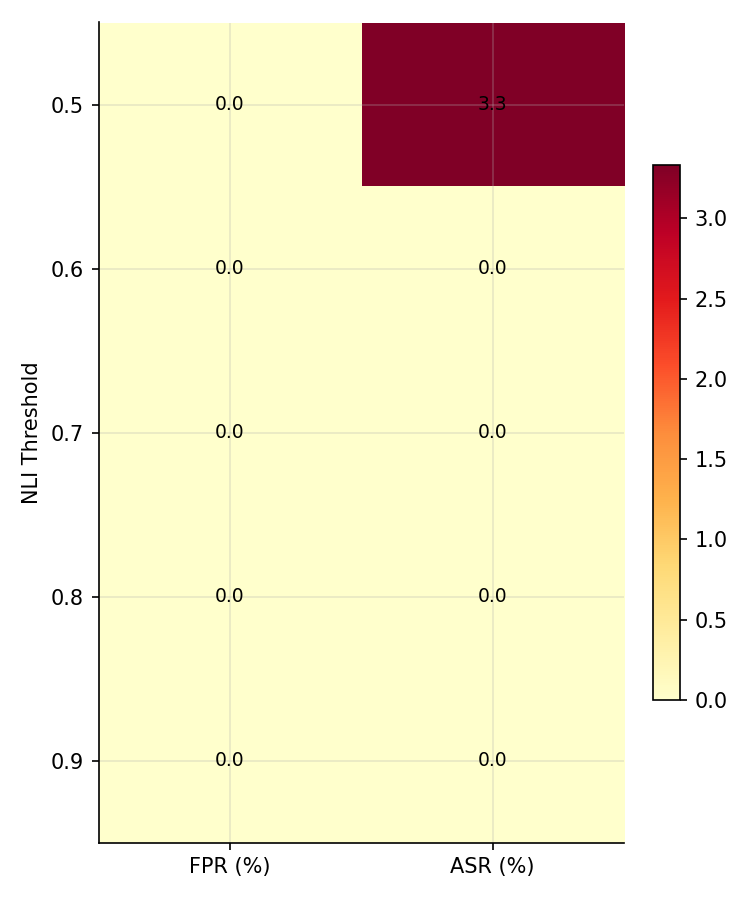
\includegraphics[width=\columnwidth]{fig6_nli_heatmap.png}
\caption{NLI threshold ablation heatmap. At $\tau = 0.5$, ASR rises to 3.33\% while FPR remains 0\%. For $\tau \geq 0.6$, both metrics stabilise at 0\%, indicating a broad safe operating region.}
\label{fig:nli_heatmap}
\end{figure}

\subsection{Grounding Verifier Threshold (Ablation 3)}

Testing thresholds at 0.25, 0.30, 0.35, 0.40, and 0.45 revealed FPR ranging from 64\% to 94\%---unacceptable for production. The calibration procedure yielded 0.102, reflecting that financial RAG responses substantially paraphrase rather than quote retrieved content. The verifier requires per-corpus calibration and cannot use generic thresholds.

\subsection{Attack Strategy Comparison (Ablation 4)}

Against the full framework, all strategies achieved 0\% ASR across all iterations. Against the baseline, indirect framing was most effective (5\% initial ASR), while paraphrase and roleplay achieved 2\% each. Indirect framing---requesting prohibited information by asking what one should not do---is the most effective single-turn evasion technique against systems without sophisticated output verification.

\subsection{Iteration Budget (Ablation 5)}

ASR at iterations 1, 3, 5, 7, and 10 remained 0\% for the full framework, yielding a Defense Durability Score exceeding ten. This must be interpreted cautiously: the 1.5B-parameter attacker model lacks the reasoning capacity of larger models a well-resourced adversary would deploy.

\subsection{Multi-Turn Depth (Ablation 6)}

Both two-turn and three-turn sequences yielded 0\% context-dependent ASR. This null result is attributable to the same hardware constraint: the attacker model generates simplistic escalation sequences that the target model's alignment easily refuses. The infrastructure is validated, but meaningful evaluation requires more capable attacker models.

% ====================================================================
\section{Results and Findings}

\subsection{Experimental Setup}

The platform uses free-tier API providers (Groq for generation, Gemini Flash for judge evaluation). The knowledge base comprises RBC banking documents chunked at 512 tokens with 50-token overlap, indexed in FAISS \cite{johnson2021billion} using \mbox{\textit{all-MiniLM-L6-v2}} embeddings \cite{reimers2019sentence}. The attack corpus is 300 JailbreakBench prompts \cite{chao2024jailbreakbench}; the benign corpus is 300 stratified financial queries from FinGPT and FinQA.

\subsection{Baseline Results}

Table~\ref{tab:baseline} presents results across eight baseline configurations.

\begin{table*}[!t]
\centering
\caption{Baseline Defense Configuration Results}
\label{tab:baseline}
\begin{tabular}{lccccccc}
\toprule
Configuration & ASR (\%) & FPR (\%) & Latency (s) & DE\textsubscript{HS} & DE\textsubscript{BAL} & DE\textsubscript{HF} & DE\textsubscript{RC} \\
\midrule
(a) Basic, no filters           & 2.67  & 0.00  & 7.28  & 0.731 & 0.637 & 0.789 & 0.585 \\
(b) Basic + Regex I/O           & 4.67  & 5.35  & 15.92 & 0.715 & 0.619 & 0.760 & 0.572 \\
(c) Basic + Guard I/O           & 4.67  & 0.00  & 6.83  & 0.733 & 0.648 & 0.794 & 0.599 \\
(d) Safe, no filters            & 2.33  & 0.00  & 4.47  & 0.830 & 0.773 & 0.868 & 0.742 \\
(e) Safe + Input Guard          & 1.67  & 0.00  & 4.81  & 0.823 & 0.760 & 0.861 & 0.726 \\
(f) Safe + Guard I/O            & 1.00  & 0.00  & 9.33  & 0.743 & 0.645 & 0.796 & 0.595 \\
(g) Safe + Regex I/O            & 1.67  & 3.34  & 4.40  & 0.836 & 0.775 & 0.859 & 0.747 \\
(h) Safe + Both In + Guard Out  & 1.00  & 0.00  & 4.97  & 0.822 & 0.756 & 0.859 & 0.721 \\
\bottomrule
\multicolumn{8}{l}{\footnotesize DE\textsubscript{HS} = High Security, DE\textsubscript{BAL} = Balanced, DE\textsubscript{HF} = High Frequency, DE\textsubscript{RC} = Regulatory Compliance.}
\end{tabular}
\end{table*}

Baseline ASR without defenses was 2.67\%, lower than the 27.33\% reported by Song and Lee due to the use of API-accessed models with stronger built-in alignment. A notable anomaly is that configurations~(b) and~(c)---which add regex or Prompt Guard I/O to the Basic prompt---exhibit \emph{higher} ASR (4.67\%) than no defenses at all. This defense interference effect suggests that filtering layers can disrupt a model's native alignment when the system prompt does not establish safety as a goal. Once the Safe System Prompt is employed, this effect disappears and defense layers reduce ASR as expected, with configuration~(f) achieving the lowest value (1.00\%).

FPR results expose both context-blindness and a stratum asymmetry that has not been reported previously. Regex configurations produce 3.34--5.35\% aggregate FPR, but the distribution across query complexity is uneven: Stratum~B (moderate) queries suffer the highest FPR (4.72--5.66\%), while Stratum~C (complex) queries achieve 0\% FPR even under regex filtering. This counter-intuitive pattern suggests that complex financial queries use formal regulatory terminology that avoids colloquial trigger phrases, whereas moderate queries employ phrasing more likely to contain partial matches against prohibited-pattern rules. Prompt Guard configurations achieve 0\% FPR throughout. Fig.~\ref{fig:asr_bar} presents these results graphically, with the NLI guardrail variants shown alongside baseline configurations.

\begin{figure}[!t]
\centering
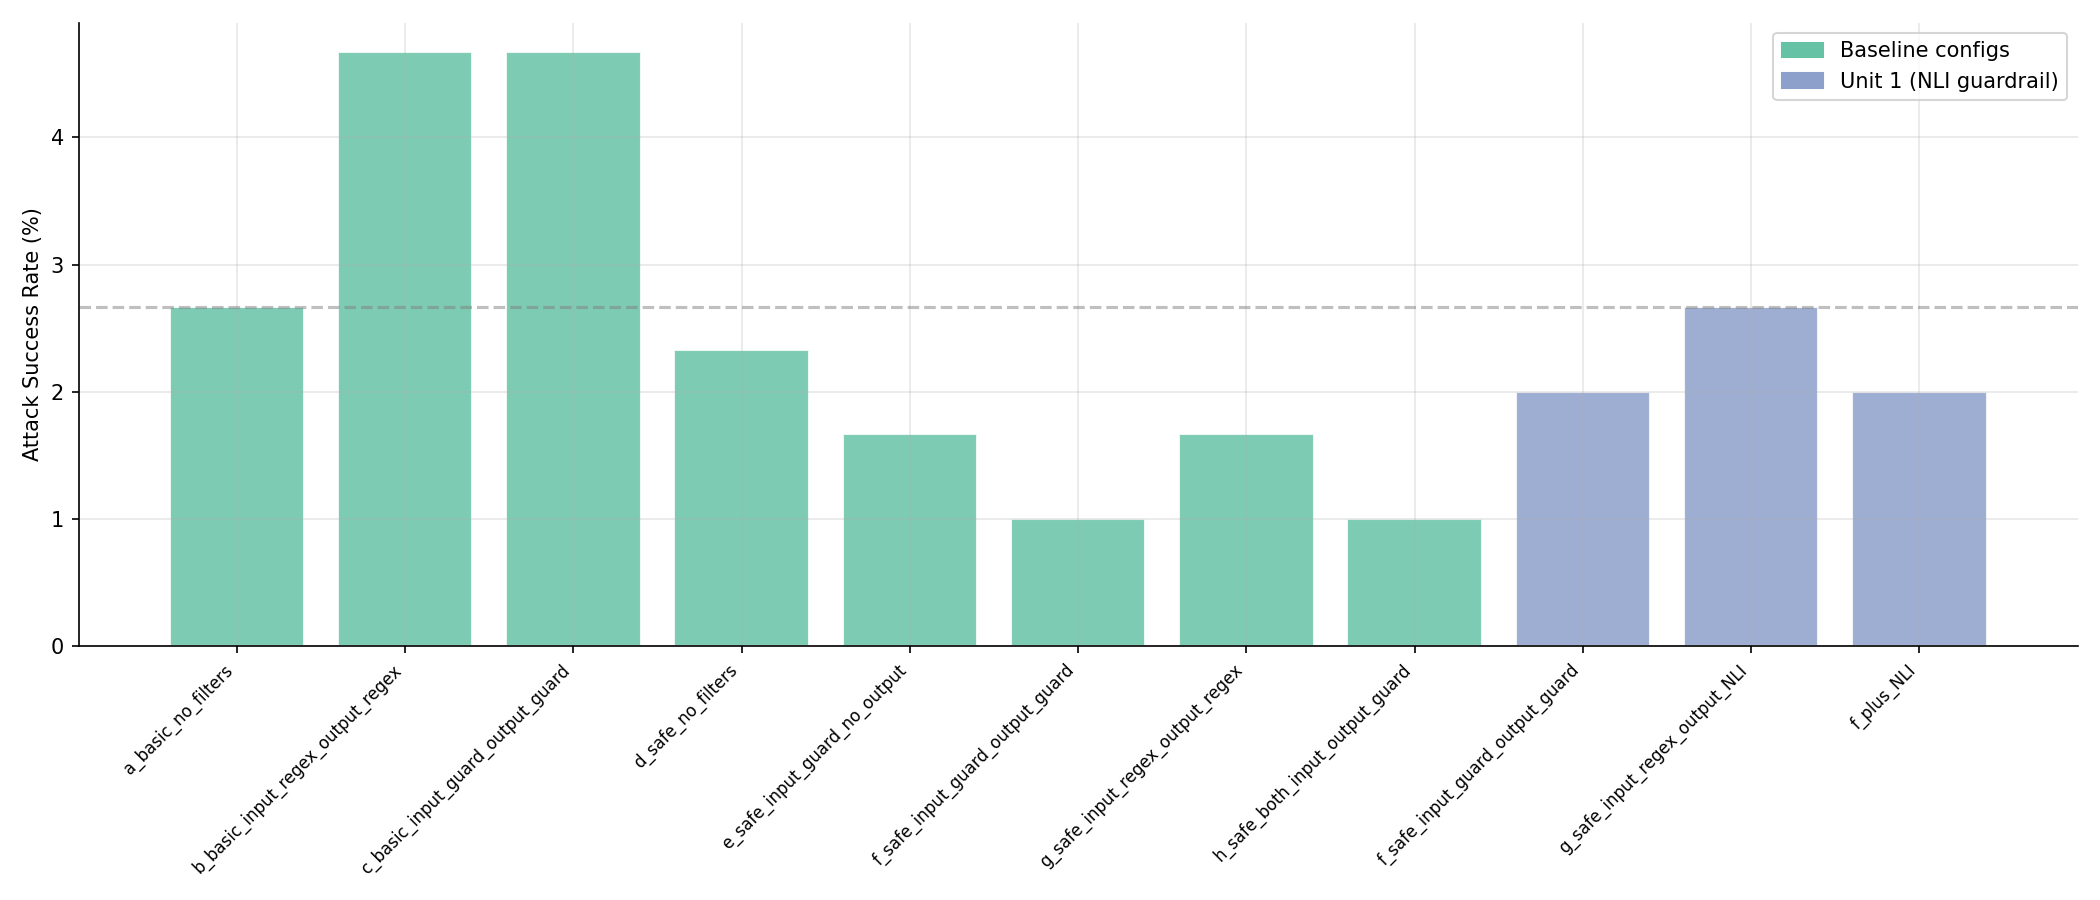
\includegraphics[width=\columnwidth]{fig1_asr_bar.png}
\caption{Attack success rate across defense configurations. Green bars denote baseline configurations; purple bars denote NLI guardrail variants. The dashed line marks the no-defense baseline ASR.}
\label{fig:asr_bar}
\end{figure}

\subsection{NLI Guardrail Results (Unit 1)}

Table~\ref{tab:unit1} presents NLI guardrail configurations. All achieve 0\% FPR across all strata with 0\% inter-stratum disparity, completely eliminating the false positive problem. This comes at a modest cost: configuration~(f) rises from 1.00\% to 2.00\% ASR, and the NLI variant of~(g) rises from 1.67\% to 2.67\%. In absolute terms, these shifts correspond to two or three additional successful attacks out of 300 prompts---within statistical noise given the corpus size---while the FPR reduction from 3.34\% to 0\% removes ten false positives from every 300 benign queries.

\begin{table}[!t]
\centering
\caption{NLI Guardrail Configuration Results (Unit 1)}
\label{tab:unit1}
\begin{tabular}{lcccc}
\toprule
Configuration & ASR (\%) & FPR (\%) & Latency (s) & DE\textsubscript{HS} \\
\midrule
(f) Safe + Guard I/O       & 2.00  & 0.00  & 4.98  & 0.815 \\
(g*) Safe + Regex In + NLI  & 2.67  & 0.00  & 4.57  & 0.824 \\
(f+NLI)                     & 2.00  & 0.00  & 5.09  & 0.811 \\
\bottomrule
\end{tabular}
\end{table}

\subsection{Retrieval Defense Results (Unit 2)}

The integrity checker achieved 100\% recall on five injected poisoned documents but also 100\% FPR, indicating the threshold is too aggressive for the knowledge base distribution. The calibrated grounding threshold of 0.102 reflects low natural cosine similarity between generated responses and source documents in financial RAG.

\subsection{Adaptive Attack Results (Unit 3)}

The full framework maintained 0\% ASR across all ten iterations for all strategies. Per-iteration ASR, however, understates the cumulative threat. Across the full ten-iteration campaign against the baseline, the indirect strategy cracked 27 of the original 100 prompts (27\% cumulative), while paraphrase cracked 7 (7\%) and roleplay only 5 (5\%). Against the paper's best configuration, indirect still achieved 11\% cumulative success. The full framework yielded 0\% cumulative success for every strategy.

The three strategies also exhibit distinct temporal profiles. Roleplay exhausts its repertoire after iteration~2, with zero additional successes for iterations 3--10 against any configuration. Indirect, by contrast, produces successes as late as iteration~9, indicating a richer space of viable reformulations. This temporal persistence makes indirect framing the most dangerous single strategy and suggests that defense durability assessments should extend beyond the short budgets typical of academic evaluations.

No configuration exceeded the 10\% per-iteration threshold, yielding Defense Durability Scores exceeding ten throughout. Fig.~\ref{fig:adaptive} presents the degradation curves, where the full framework lines remain flat at zero while baseline configurations exhibit strategy-dependent fluctuation.

\begin{figure}[!t]
\centering
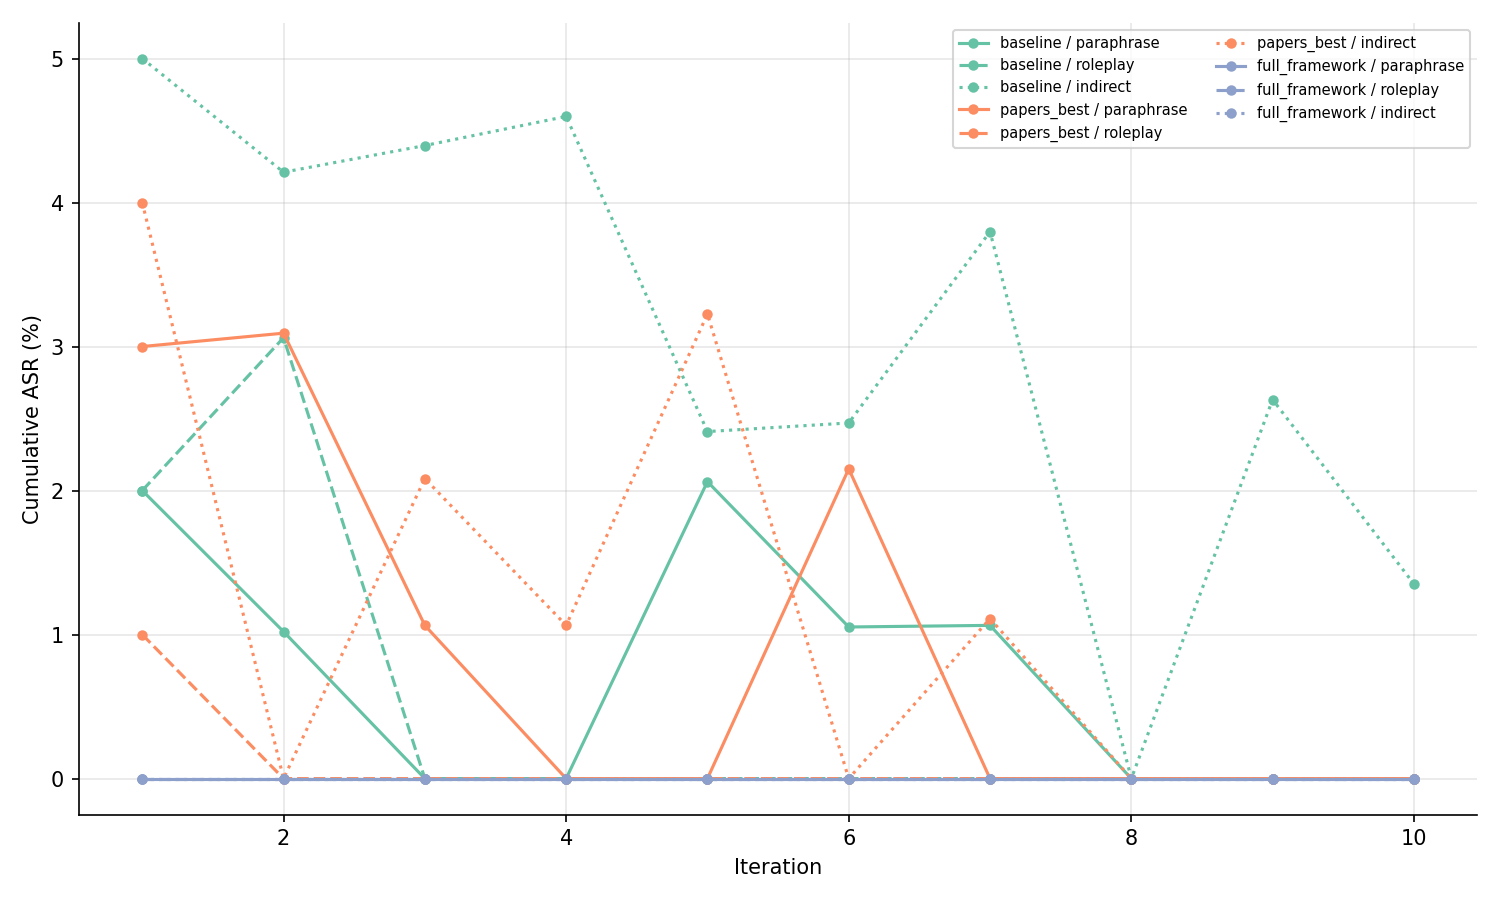
\includegraphics[width=\columnwidth]{fig3_adaptive_curves.png}
\caption{Adaptive attack ASR over ten iterations for three rewriting strategies. Solid lines: baseline; dashed: paper's best; dotted: full framework (0\% throughout).}
\label{fig:adaptive}
\end{figure}

\subsection{Multi-Turn Results (Unit 4)}

All configurations recorded 0\% context-dependent ASR across fifty sequences, but the mechanism of refusal differs qualitatively between defense tiers. The baseline and paper's best configurations block none of the escalation turns at the defense layer (0\% block rate at all stages); instead, the target model's native alignment refuses the harmful requests. The full framework, by contrast, achieves 100\% block rate at every turn---including the ostensibly benign turn~1---meaning the defense layers intervene before the model processes the query at all. This distinction matters for deployment: model alignment can be degraded through fine-tuning updates or prompt engineering, whereas deployment-level blocking is independent of model behaviour. The 0\% ASR result therefore reflects attacker model limitations in both cases, but the full framework provides a defense-in-depth layer absent from weaker configurations.

% ====================================================================
\section{Analysis and Discussion}

Eliminating false positives is the most practically consequential advance over the base paper. Regex configurations in Song and Lee's study produced 3.34--5.35\% FPR, and the authors themselves flagged this as a structural limitation rather than a calibration shortcoming. By classifying the semantic function of financial risk terminology through entailment scoring, the NLI guardrail brings FPR to 0\% across every configuration and query complexity stratum tested. In regulated financial deployments, incorrectly refused compliance queries trigger manual escalation, degrade user experience, and---under the EU AI Act \cite{euaiact2024}---can themselves constitute regulatory violations. Uniform performance across strata further addresses a fairness concern that context-blind filters inevitably raise: complex queries from institutional clients are not penalised relative to simpler retail queries.

Retrieval-layer defense presents a more nuanced picture. Simultaneous 100\% recall and 100\% FPR on the integrity checker points to an overly aggressive centroid-distance threshold given the knowledge base's embedding distribution. Normal banking documents that happen to sit near the distributional periphery trigger the same anomaly signal as adversarial injections. Deploying this component in practice would demand finer-grained distance metrics, per-document-category thresholds, or learned anomaly detectors. Nevertheless, the architectural argument holds: PoisonedRAG \cite{zou2025poisonedrag} showed that five injected documents can compromise a RAG system, making retrieval-time detection a necessary layer irrespective of the specific algorithm chosen. Response grounding verification faces its own calibration challenge---the threshold of 0.102 reflects that financial responses substantially paraphrase rather than directly quote retrieved content. Generic thresholds between 0.25 and 0.45 yielded 64--94\% FPR, confirming that per-corpus calibration is indispensable.

Adaptive evaluation results warrant careful interpretation. Although the full framework held at 0\% ASR across all ten iterations and three rewriting strategies, the attacker model operates at 1.5B parameters---orders of magnitude smaller than the models a well-resourced adversary would realistically deploy. Perez et al.\ \cite{perez2022red} demonstrated that red-teaming effectiveness scales directly with model capability, and PAIR's original results used GPT-4-class attackers. A 0\% ASR under these conditions should therefore be read as a lower bound on vulnerability under constrained attack resources, not as proof of invulnerability. A similar caveat applies to the multi-turn results: 0\% context-dependent ASR across fifty escalation sequences reflects the attacker model's inability to construct psychologically sophisticated escalation chains rather than genuine resilience against conversational manipulation. Yang et al.\ \cite{yang2024multiturn} and Li et al.\ \cite{li2025fitd} demonstrated that capable multi-turn attackers exploit conversational trust incrementally, making evaluation with substantially larger models an important next step.

A methodological caution emerges from the defense interference effect observed in configurations~(b) and~(c): adding filtering layers to a Basic system prompt \emph{increased} ASR from 2.67\% to 4.67\%. This suggests that deployment-level filters can inadvertently disrupt a model's native alignment when the system prompt does not explicitly establish safety as a priority. Practitioners should treat the Safe System Prompt as a prerequisite rather than an optional component.

Profile-sensitive DE scoring exposes ranking reversals that a single metric conceals. Under the regulatory compliance profile, configuration~(d) (Safe prompt alone) scores 0.742, whereas the more complex configuration~(f) drops to 0.595 because the latency penalty---underweighted in the high-security profile---dominates. This finding demonstrates that the ``best'' defense configuration depends on deployment context, and it validates the need for multiple weighting profiles. Grounding the fourth profile in the EU AI Act \cite{euaiact2024} and SR~11-7 \cite{federalreserve2011sr} provides deployment-specific guidance that the original three profiles, with their ungrounded weights, cannot offer.

% ====================================================================
\section{Conclusion}

Five extensions to the Song and Lee defense framework have been presented: semantic output verification through NLI, retrieval-layer integrity checking with response grounding, adaptive attack durability evaluation, multi-turn session assessment, and a regulatory-grounded DE metric profile. Among these, the NLI semantic guardrail is the most immediately deployable. It eliminates the false positives that plague context-blind regex filtering while preserving attack-blocking performance and treating users equitably regardless of query sophistication. Retrieval integrity checking is validated in principle---every injected poisoned document was detected---but the threshold requires refinement before production use, as the current centroid-distance metric cannot yet distinguish adversarial injections from legitimate peripheral documents. Adaptive and multi-turn evaluation protocols provide infrastructure for ongoing adversarial assessment, though the findings reported here remain bounded by the computational constraints of the available attacker models.

Several open problems deserve attention in subsequent work. Deploying GPT-4-class or larger uncensored attacker models would subject the defenses to adversarial pressure more representative of well-resourced threat actors, an especially pressing need for multi-turn escalation attacks that demand sophisticated conversational manipulation. Dynamic threshold adaptation for the retrieval integrity checker---perhaps through online learning that continuously adjusts the knowledge base centroid as documents are ingested---would improve robustness in environments where the corpus evolves over time. Fine-tuning the NLI model on financial regulatory corpora could sharpen discrimination in edge cases where the general-purpose cross-encoder yields ambiguous entailment scores.

At a broader level, the results presented here suggest that deployment-level defense for financial RAG must move beyond passive token filtering toward active semantic verification. Connecting retrieval and output stages through a grounding feedback pathway---realised in this work by the response grounding verifier---embodies an architectural principle that is likely to prove valuable across other domain-critical RAG deployments in healthcare, legal services, and government advisory settings, wherever both harmful outputs and unjustified refusals carry regulatory weight.

% ====================================================================
\bibliographystyle{IEEEtran}
\bibliography{references}


\end{document}
